\documentclass[a4paper,12pt]{article}
\usepackage{tabularx}
\usepackage{hyperref}
\usepackage{multirow}
\usepackage{graphicx}
\usepackage{caption} 
\usepackage{amsmath}


\title{Heating task Report}
\author{Macarena Burguera Perello(\textit{s243296}), \\
        Levente Buzga (\textit{s242964}), \\
        Attila István Kiri (\textit{s242965})}


\begin{document}

\maketitle


\section{Introduction}

In this report, we present the development and optimization of a Python-based simulation designed to evaluate the effectiveness of the Wall Heating concept, as part of the 02613 Python and High-Performance Computing course mini-project. Our primary objective is to create a solution that is both scalable and computationally efficient, enabling rapid evaluation across a large dataset. While we address all the questions outlined in the project description, some tasks are combined where it improves clarity and cohesion.

\section{Tasks}

In this project, we focus on developing and optimizing a Python-based simulation to evaluate the effectiveness of a novel heating method called Wall Heating, which uses interior walls as heat sources. Using the Modified Swiss Dwellings dataset, we simulate heating performance across thousands of building floorplans while prioritizing efficient code execution. The main goal is to ensure that our implementation is both scalable and computationally efficient to enable rapid evaluation across a large dataset.

\subsection{Task 1}

The data provided in the Modified Swiss Dwellings dataset is in a npy format, which is a numpy array format. To load the data we created a python script that uses the numpy library.
Each building has an ID which is stored in \texttt{building\_ids.txt}, 
and two corresponding to the floor plan:

Interior: This file contains a NumPy array with a binary mask. It is 1 for all
interior grid points (i.e., grid points inside a room) and 0 for all other grid points (i.e., grid points
on walls and outside the building
And one for the heating 

Domain: This file contains a NumPy array with the initial conditions for the
simulation grid u. Grid points on load bearing walls have been been set to 5 and grid points on
inside walls to 25. All other points have been set to 0.
This is shown in Figure~\ref{fig:combined_plot}.

\begin{figure}[h!]
        \centering
        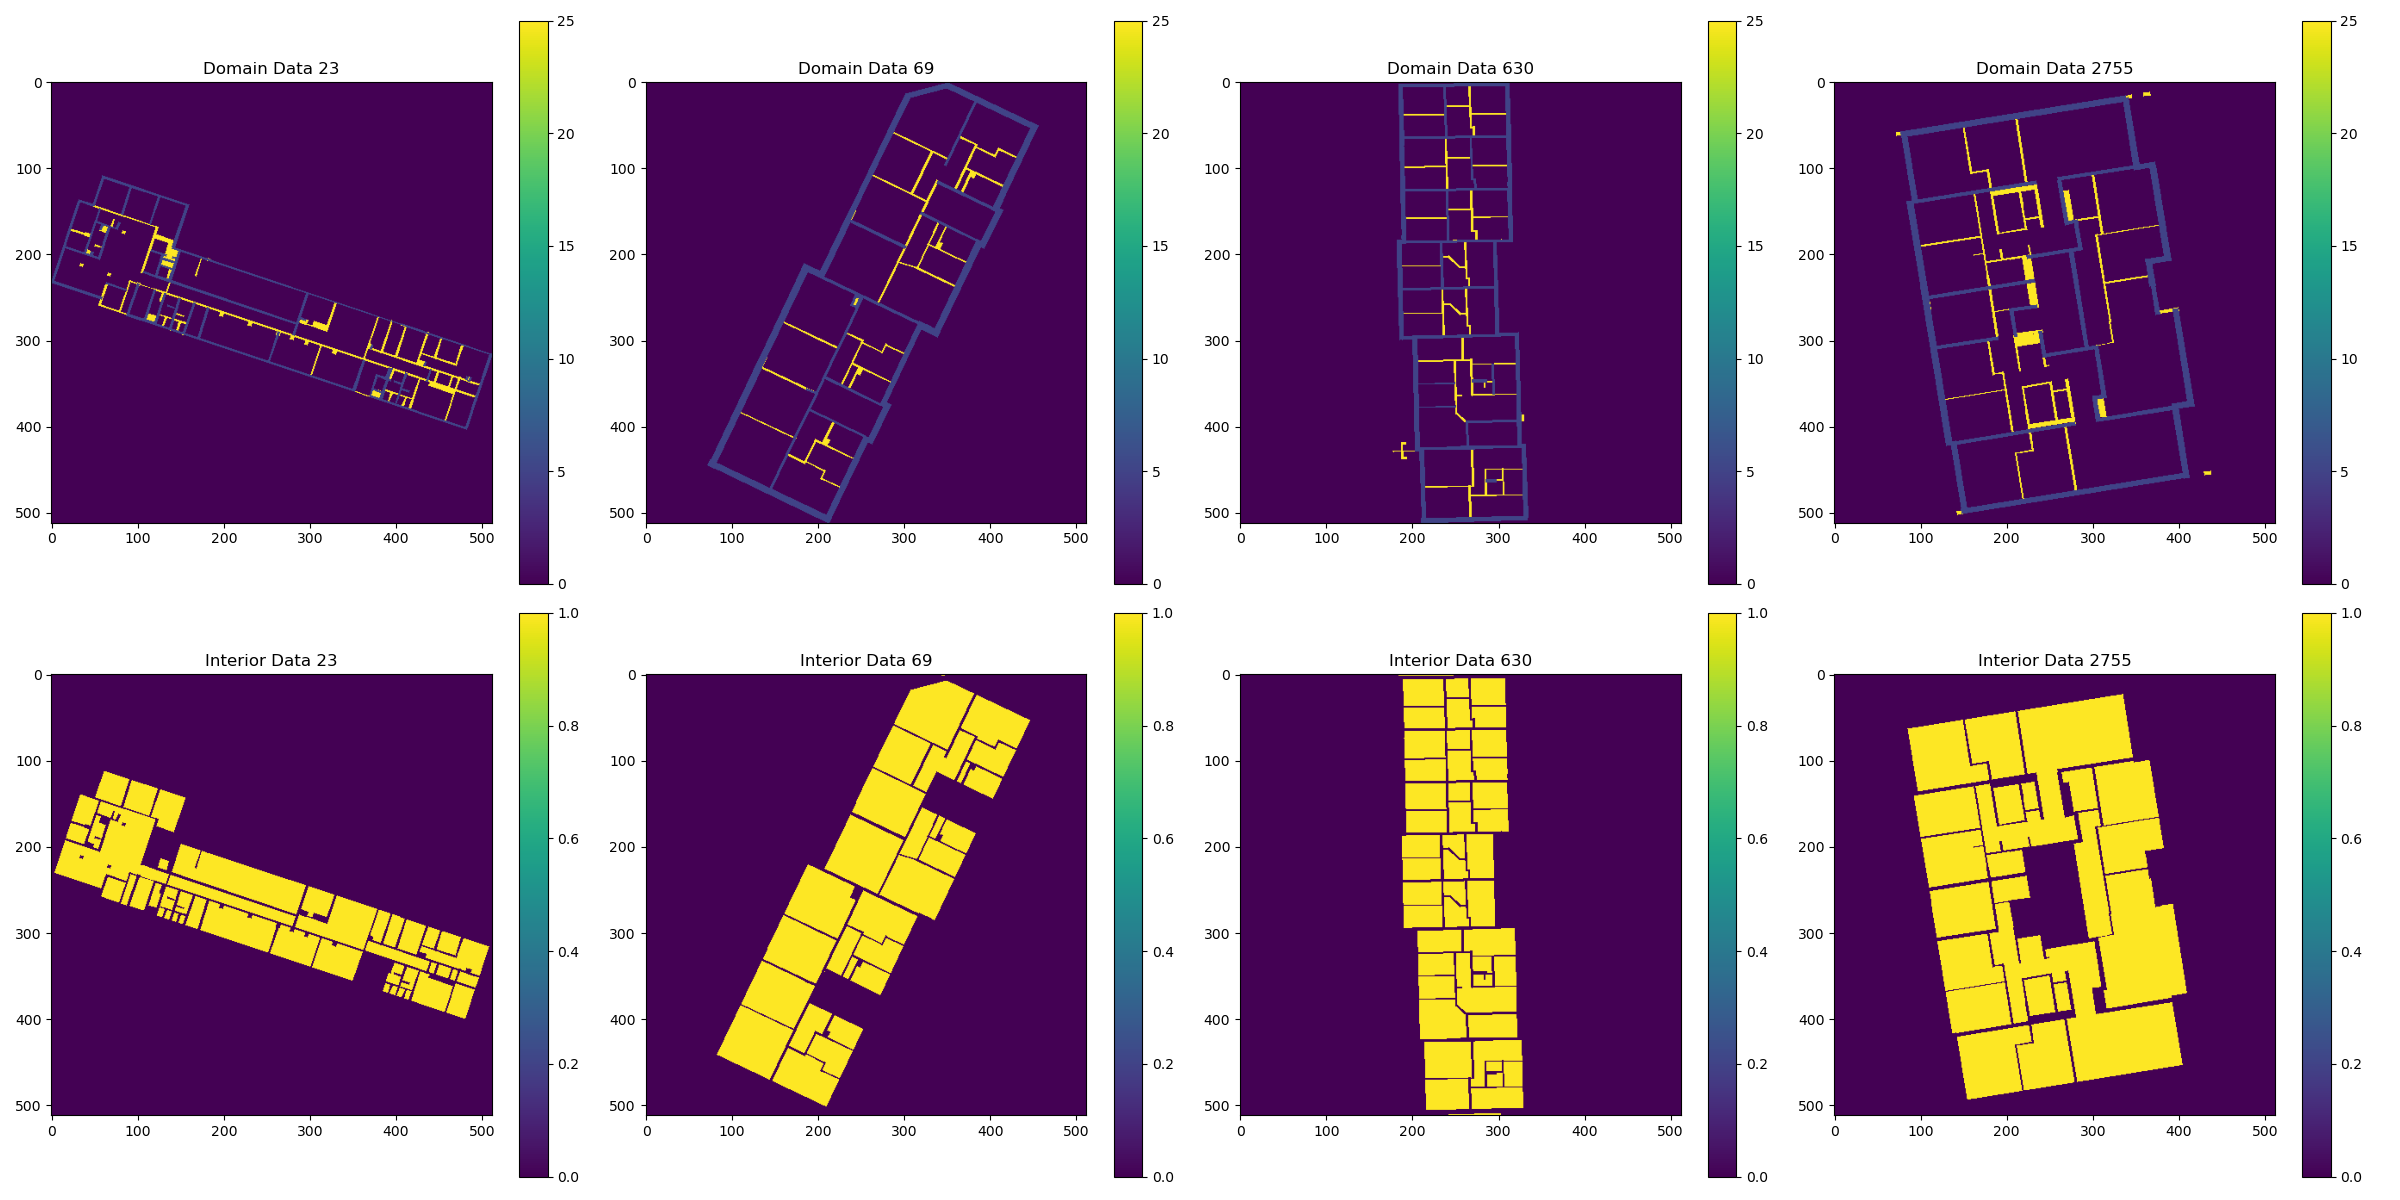
\includegraphics[width=1\textwidth]{Plots/combined_plot.png}
        \caption{Visualization of the dataset: Building IDs, floor plans, and heating domains.}
        \label{fig:combined_plot}
\end{figure}

\subsection{Task 2}
When trying to run the simulation on 20 input files, we timed around 215 seconds. We know there is 4571 different building IDs which means the program should be ran for that amount of times which if we take our previous time it would be estimately:
\[
\text{Total time for 4571 buildings: } T_{\text{total}} = \frac{4571}{20} \times 215
\]

\[
T_{\text{total}} = 49191.25 \text{ seconds} = 819.85 \text{ minutes} = 13.66 \text{ hours}
\]
This shows that the simulation is not efficient enough to run on a large dataset. We need to optimize the code to reduce the time taken for each simulation.


\subsection{Task 3}
Now that we ran the simulation we can start analyzing the results. In the output we can find 4 different metrics that characterizes the heating performance of the building. These are:

\begin{itemize}
        \item The \textbf{mean temperature} and a corresponding \textbf{standard deviation} across the floor plan. This is shown in Figure~\ref{fig:temperature_distribution}.

        \begin{figure}[h!]
                \centering
                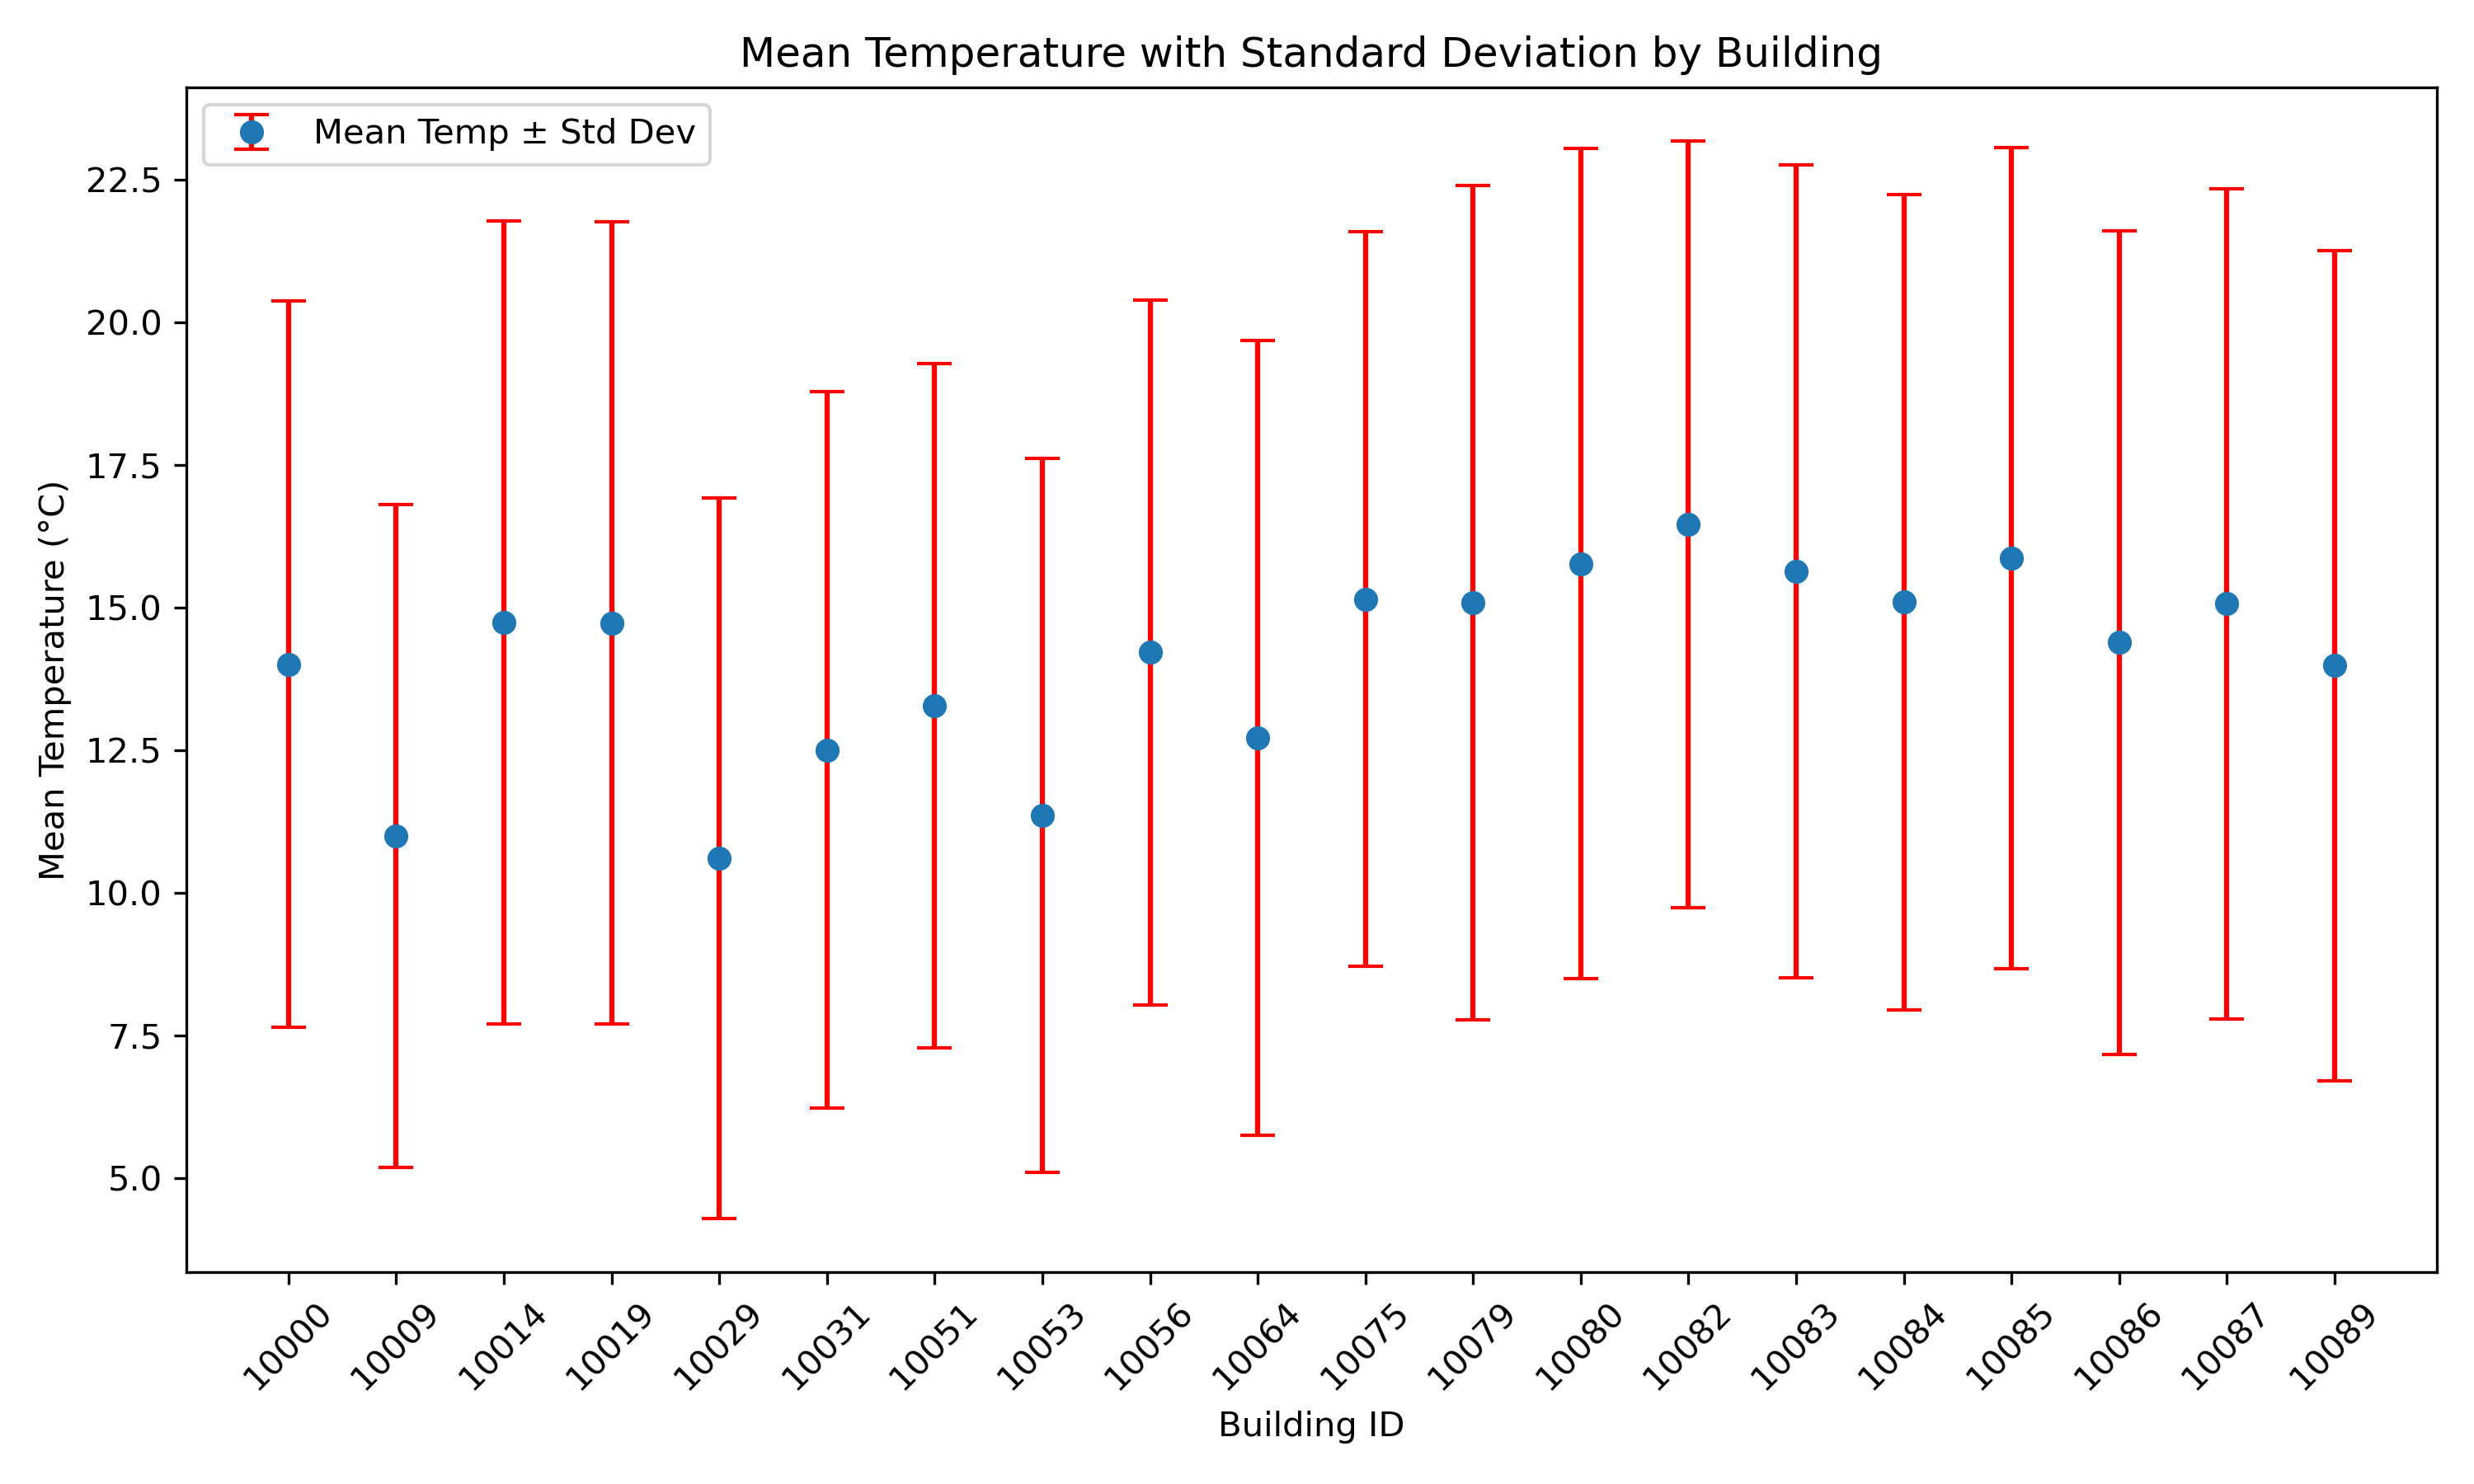
\includegraphics[width=1\textwidth]{Plots/mean_temp_with_std_dev.png}
                \caption{Temperature distribution across the 20 floor plans.}
                \label{fig:temperature_distribution}
        \end{figure}

        \item Areas with temperatures above 18ºC are considered safe from mold risk.
        \item Areas with temperatures below 15ºC are deemed too cold for human comfort, as seen on Figure~\ref{fig:temperature_distribution_precentage}.
        \begin{figure}[h!]
                \centering
                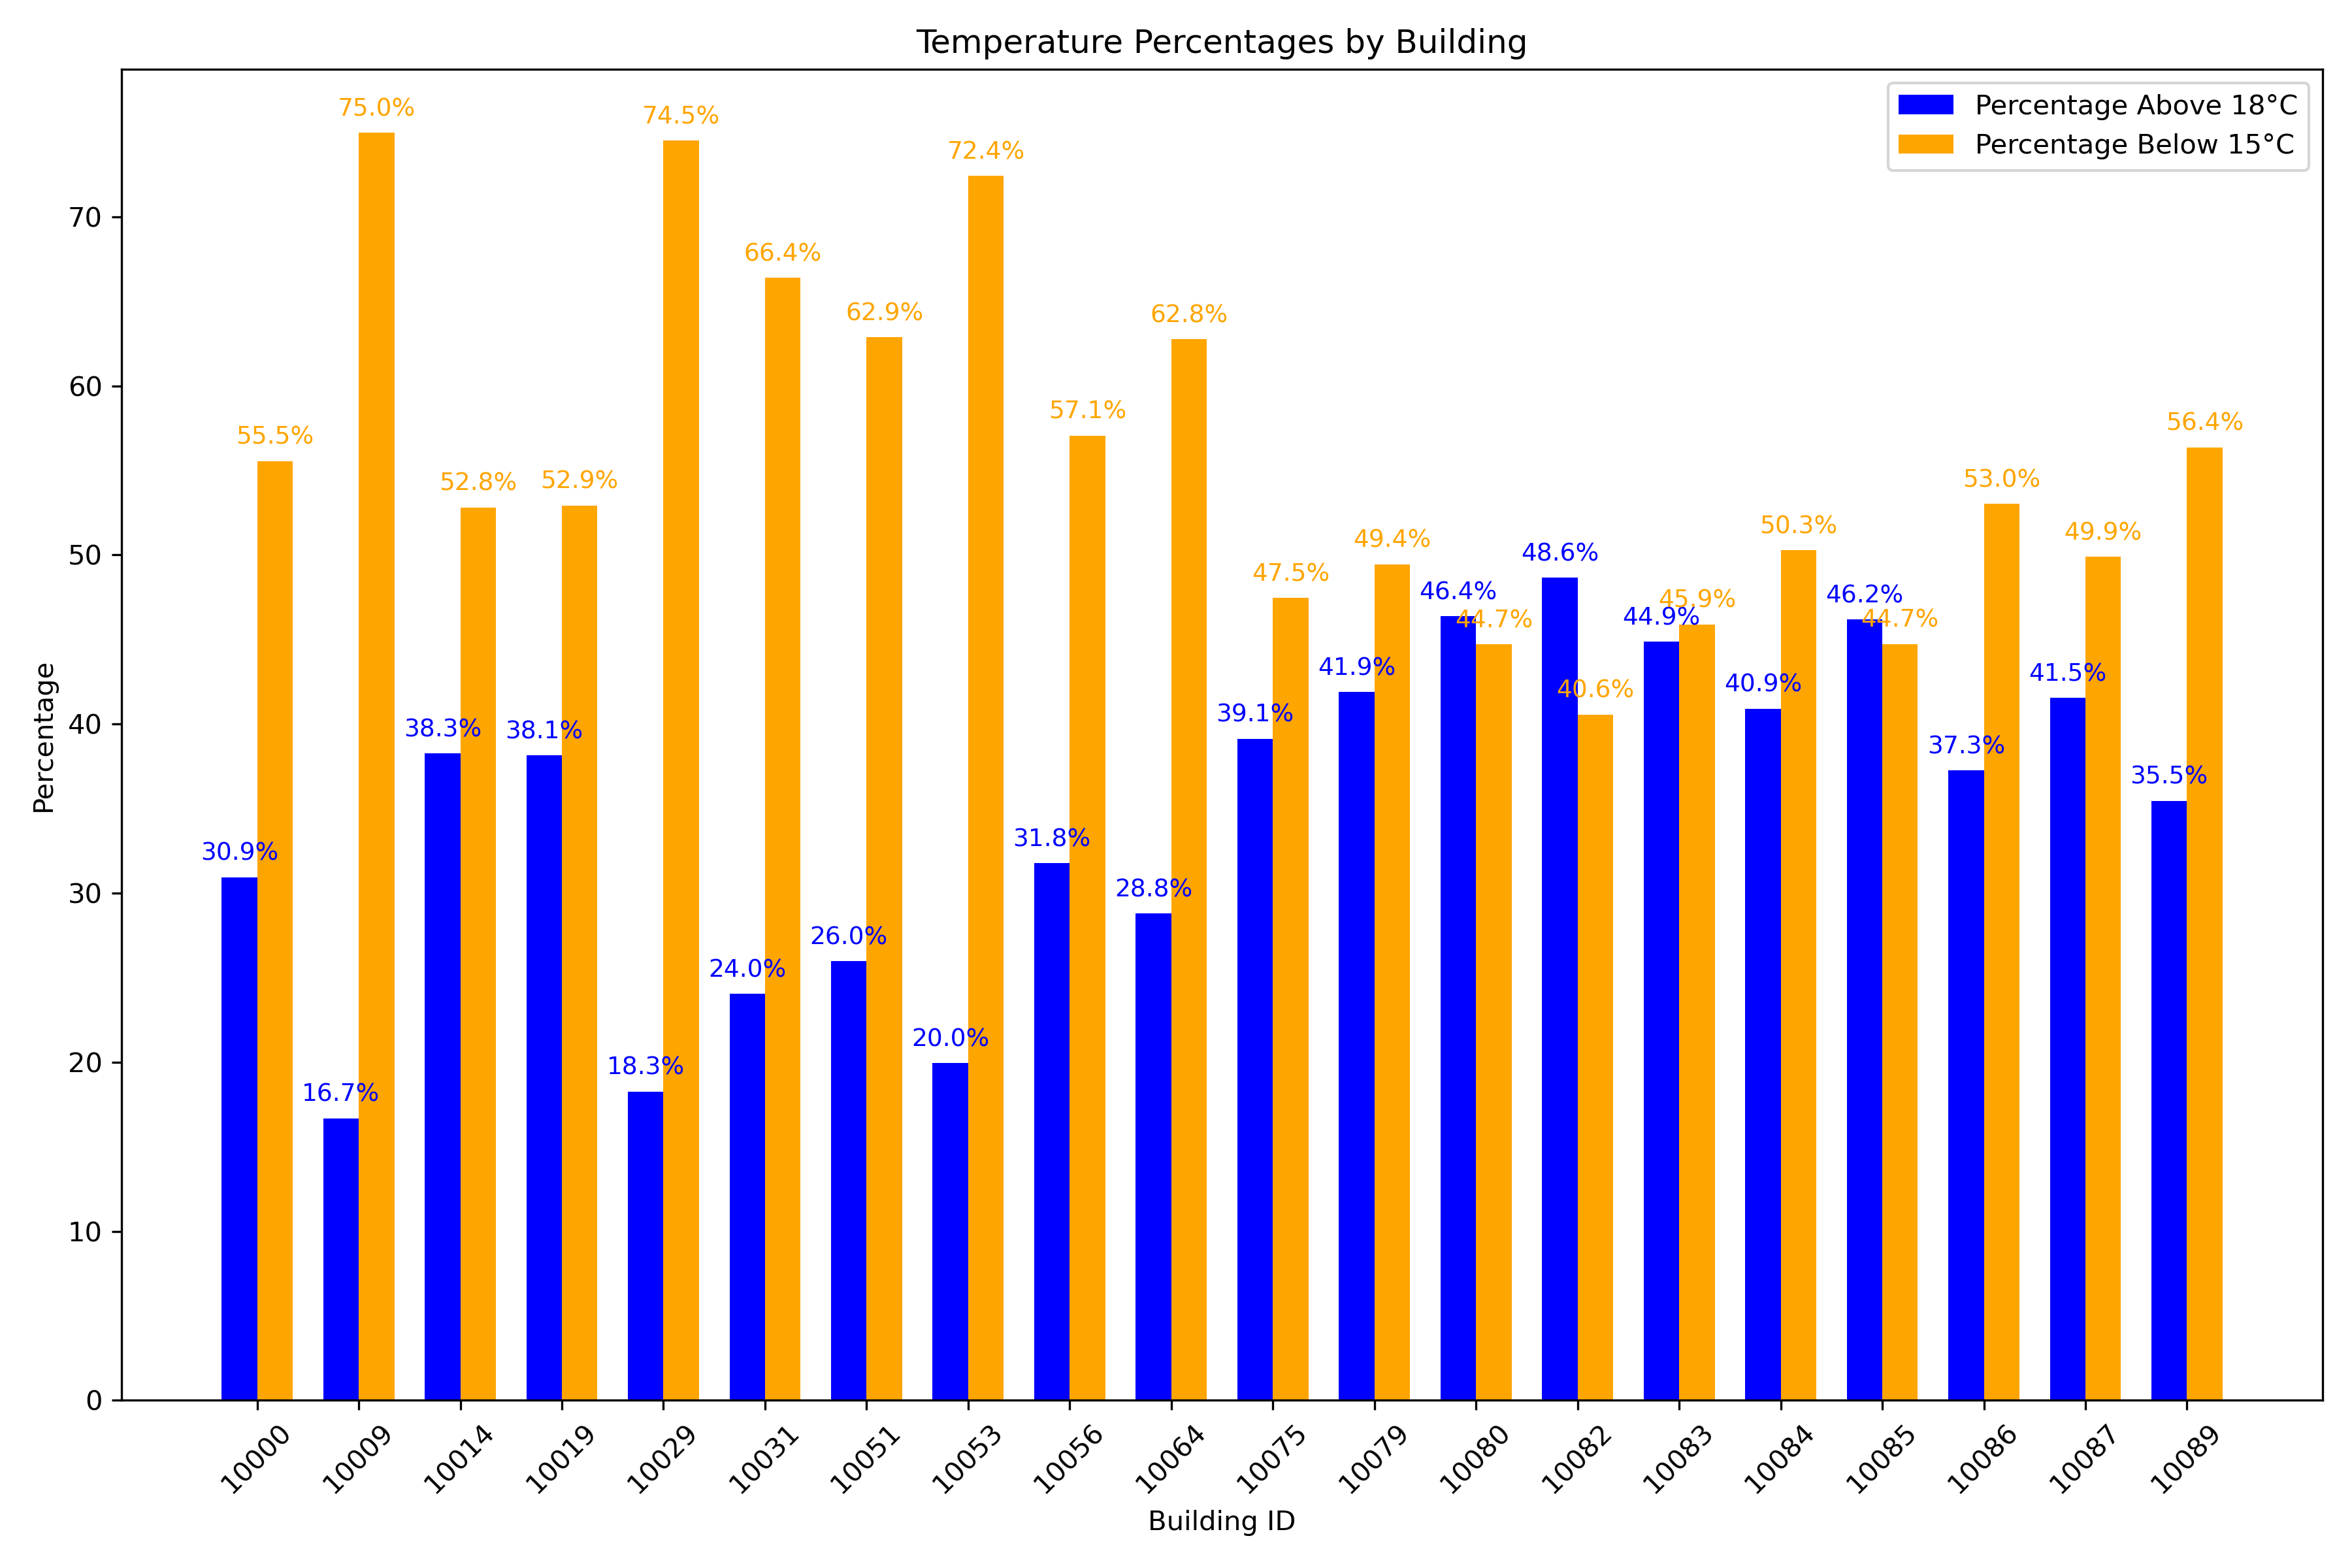
\includegraphics[width=1\textwidth]{Plots/temperature_percentages_by_building.png}
                \caption{Percentage of areas with different temperatures across the 20 floor plans.}
                \label{fig:temperature_distribution_precentage}
        \end{figure}

\end{itemize}


\subsection{Task 4}

Profile the reference jacobi function using kernprof. Explain the different parts of the function and how much time each part takes

\subsection{Task 5}

Make a new Python program where you parallelize the computations over the floorplans. Use static scheduling such that each worker is assigned the same amount of floorplans to process.

You should use no more than 100 floorplans for your timing experiments. Again, use a batch job to ensure consistent results.
a) Measure the speed-up as more workers are added. Plot your speed-ups.
b) Estimate your parallel fraction according to Amdahl's law. How much (roughly) is paral-lelized?
c) What is your theoretical maximum speed-up according to Amdahl's law? How much of that did you achieve? How many cores did that take?
d) How long would you estimate it would take to process all floorplans using your fastest parallel solution?

\subsection{Task 6}
The amount of iterations needed to reach convergence will vary from floorplan to floorplan. Re-do your parallelization experiment using dynamic scheduling.

a) Did it get faster? by how much?
b) Did the speed-up improve or worsen?

\subsection{Task 7}
Implement an.other solution where you rewrite the jacobi function using Numba JIT on the CPU.

a) Run and time the new solution where you rewrite the jacobi function using Numba JIT on the CPU

a) Run and time the new solution for a small subset of floorplans. How does the performance compare to the reference?
b) Explain your function. How did you ensure your access pattern works well with the CPU cache?
c) How long would it now take to process all floorplans?

\subsection{Task 8}
Implement another solution writing a custom CUDA kernel with Numba. To synchronize threads between each iteration, the kernel should only perform a single iteration of the Jacobi solver. Skip the early stopping criteria and just run for a fixed amount of iterations. Write a helper function which takes the same inputs as the reference implementation (except for the atol input which is not needed) and then calls your kernel repeatedly to perform the implementations.
a) Briefly describe your new solution. How did you structure your kernel and helper function?
b) Run and time the new solution for a small subset of floorplans. How does the performance compare to the reference?
c) How long would it now take to process all floorplans?

\subsection{Task 9}
Adapt the reference solution to run on the GPU using CuPy.
a) Run and time the new solution for a small subset of floorplans. How does the performance compare to the reference?
b) How long would it now take to process all floorplans?
c) Was anything surprising about the performance?

\subsection{Task 10}
Profile the CuPy solution using the nsys profiler. What is the main issue regarding performance? (Hint: see exercises from week 10) Try to fix it.

\subsection{Task 11}
(Optional) Improve the performance of one or more of your solutions further. For example, parallelize your CPU jIT solution. Or use job arrays to parallelize a solution over multiple jobs. How fast can you get?

\subsection{Task 12}
Process all floorplans using one of your implemtnations (ideally a fast one) and answer the below questions.
Hint: use Pandas to process the CSV results generated by the script
a) What is the distribution of the mean temperatures? Show your results as histograms.
b) What is the average mean temperature of the buildings?
c) What is the average temperature standard deviation?
d) How many buildings had at least 50 per cent of their area above 18º?
e) How many buildings had at least 50 per cent of their area below 15º?


\end{document}